\section{Detailed Implementation}

\label{sec:implement}

\section{Implementation}


\input{implement-stefen}
\input{implement-sam}

\subsection{Understanding Different Allocators}

\label{sec:understandingallocators}

\MP{} relies on a ``prerun'' program to understand the details of different allocators, such as the allocator's style (BIBOP versus bump-pointer-based), class sizes, the threshold separating small objects from large objects, and an approximate size of metadata per object. 

In order to identify the various class sizes, the prerun routine begins by allocating an object of 8 bytes, and continues to allocate  additional objects using a stepped increase of 8 bytes each time. For BIBOP-style allocators, we confirm whether objects are allocated from within different pages to detect when the allocation of an object has been moved to a different location (i.e., another bag). 
For bump-pointer-based allocators, such as the glibc allocator, we confirm size classes by checking the proximity of contiguously allocated objects of distinct sizes, and observing whether a significant address difference exists between the placement of these objects. For example, if an 8 byte object is located immediately adjacent to a 512 byte object, this is typically a strong indication that the allocator utilizes a bump-pointer-based object management style.
%Open BSD's allocator ``reverse aligns'' objects that are between 2Kb and 4Kb in size. The allocator aligns the objects last byte to the end of the page in which it resides, so that the object starting byte is somewhere in the middle. The prerun would see the address change and believe it has found a new class size. Open BSD provides a flag to turn this behavior off, however this is one example of the challenges of making the profiler general purpose.

%There are many challenges in searching for metadata. Different allocators employ completely different methods in storing metadata for it's internal use. There are a number of ways we attempt to get metadata size for each object. For a bibop allocator, it's metadata has a good chance of being located in a private memory region returned from mmap. The prerun detects the mmap and checks to see if it was used to fulfill a memory request. If it wasn't we will search it for metadata. The prerun library utilizes the /proc/pid/pagemap file to identify the virtual pages which are backed by physical frames. The prerun searches the entire mmap region for physically backed virtual pages, remembering their page numbers in relation to the mmap region starting address. Finally, the prerun counts the number of non-zero bytes on all physically-backed virtual pages, using the minimum of all these values as an estimated metadata size. This method works with the assumption that the bibop-style allocator \emph{is} placing it's metadata in mmap memory. One of the allocators we tested, Dieharder, does mmap memory that was not used for allocations nor metadata, however the prerun includes these regions in it's search for metadata incorrectly. Additionally, the actual metadata is interpreted differently for different allocators. One allocator can store primitive data types in it's metadata, while another allocator uses bitmaps or byte values that have specific meaning only to that allocator. The numerous ways of storing and interpreting metadata is a huge challenge for us.
		
%Another huge challenge in the profiler is globally storing data that is thread specific in a way that is quickly accessed and synchronized between threads. There's no getting around all threads needing to access some type of global data. Doing this efficiently is a priority for the profiler. Detecting memory blowup requires the allocating thread to be aware of other threads free object status. An internal global free list of objects has too much contention from threads simultaneously inserting, deleting, and searching the free list. We employ a semi-thread local approach. Each thread has a thread local count of free objects (by class size for bibop) and the profiler maintains one global count (again by class size for bibop). When a thread allocates, there are three possibilities that we check in determining memory blowup, always starting with the thread checking it's thread local free count. If the thread has free objects it can reuse, the profiler assumes that the thread will reuse one of it's free objects, and decrements its local and global counter. If the thread does not have free objects, it checks to see if there are free objects globally. If there are, the profiler accounts for that one occurrence of memory blowup and decrements the global counter. The last situation is that the thread does not have any free objects, and the global counter is at zero. There is no memory blowup in this situation. The global counter is synchronized using atomic accesses. This is accurate and fast method the profiler uses in detecting memory blowup. Balancing the profiler with accurate synchronized global data and performance is a huge challenge.

\subsection{Profiling Performance Overhead}

Performance overhead is profiled using several measures which, when viewed together, help to describe the performance profile of a particular allocator/application pairing.

First, as virtually all allocators treat new and reused objects differently, we differentiate between these execution paths in order to understand how each allocator differs with regard to allocation efficiency when reusing a previously freed object versus a new one. Timestamps taken both before and after each such execution pathway are compared in order to determine the total number of cycles spent within each path.

We differentiate between used and new objects differently for BIBOP-style allocators and bump-pointer-based ones. For the former, counter arrays are used to track the number of free objects for each class size used by the allocator. In this way, if the given class size free-object-counter is non-zero, we will count the executed cycles toward the ``reused object'' pathway.

Similarly for bump-pointer-based allocators, a simple running total is maintained for freed objects, and this total is compared to the size of the current allocation request.

%We differentiate the big objects and small objects. 

\subsection{Profiling Memory Overhead}
\MP{} profiles allocator memory overhead using three measures, each tracked both on both a global and per-thread basis. These measures are: maximum real memory usage, maximum real allocated memory usage, and maximum total memory usage.

\subsubsection{Real Memory Usage}
This value represents the amount of memory actually requested (and presumably being used) by the application. This is adjusted throughout runtime using the direct values provided to the allocator from the application itself. For example, if the application performs a call to \texttt{malloc(454)}, then the ``real memory usage'' parameter is correspondingly incremented by $454$.

\subsubsection{Real Allocated Memory Usage}
``Real allocated memory usage'' refers to the memory usage of the allocator, given that the user-requested size will often be placed in the nearest-fitting container, and thus will often also contain some unused slack space. For example, given a call to \texttt{malloc(454)}, a power-of-two-style BIBOP allocator will utilize a 512-byte bag from which to satisfy this request. In this instance, the class size of the requested object, $512$, will be used to increment the ``real allocated memory usage'' counter.

\subsubsection{Total Memory Usage}
``Total memory usage'' refers to the total actual physical memory dedicated to backing the objects served from the heap. To continue with the previous example, given a call to \texttt{malloc(454)}, the ``total memory usage'' counter will be incremented by the system page size (e.g. 4096 bytes), provided that the page was previously unused. Tracking of page and cache line usage is described in more detail in Section~\ref{sec:fastlookup}.

Finally, in order to track their maximal values, each time any of these measures is incremented, \MP{} will simply perform a check to determine whether the newly adjusted value exceeds its respective previously stored maximal value.

\subsection{Profiling Scalability}
Allocator scalability is evaluated by \MP{} using a variety of metrics to indicate its ability to scale well. The tracked parameters include the number various lock types (i.e., pthread mutex locks, spin locks, and try locks), as well as the maximum contention observed on each individual lock.
Further, both the number and wait cycles associated with common allocator-related system calls are tracked, including \texttt{mmap}, \texttt{munmap}, \texttt{mremap}, \texttt{sbrk}, \texttt{madvise}, and \texttt{mprotect}.

Lastly, memory blowup also has an effect on an allocator's scalability (e.g., an allocator that exhausts physical memory will not be considered to scale as well as others that do not). To this end, \MP{} tracks allocator memory blowup, but does so slightly differently for both BIBOP-style and bump-pointer-style allocators.

For BIBOP-style allocators, thread local counts of freed objects for each supported size class are maintained, as well as corresponding global counters as well. Upon an allocation request, if the current thread does not possess any freed objects of the given size class -- but if the global counter does -- we record this event as an allocation responsible for increasing the allocator's memory blowup.

Similarly, for bump-pointer-style allocators, a global counter is used to track the number of freed bytes, rather than freed objects. If the current allocation request cannot be fully satisfied from the available freed bytes, the allocator will thus utilize unused memory from the top of the heap in order to fulfill the allocation request, therefore increasing memory blowup as well.


\subsection{Application Friendliness}
Application friendliness is characterized by how well a particular allocator makes use of resources when paired with a given application, but which may also provide a pattern of usage that may be generalized across multiple applications as well.

This information includes characteristics such as (1)~the number of cache line accesses on heap data; (2)~the average cache line utilization; (3)~the average page utilization; (4)~the number of cache line writes to heap objects; and (5)~the number of cache line writes featuring an owner conflicts (i.e., a thread writes to a cache line ``belonging to'' another thread).

These data are collected using a PMU-based memory access sampling mechanism, configured with a default sampling period of 500 (plus or minus 10\%, randomly), determined at thread creation.

\subsection{Optimizations}

\subsubsection{Designing the Fast Lookup}

\label{sec:fastlookup}

As described before, \MP{} requires the size of actual allocations in order to compute the actual memory overhead. To achieve this target, \MP{} needs to maintain the size information of heap objects so that it could increment and decrement the size of objects. Another reason is that \MP{} will compute the cache fullness and page fullness for application friendliness. Thus, \MP{} also require the size information of objects to update the cache line information and page information. This indicates that \MP{} has to operate the size information upon allocations and deallocations, and on every sampled event, which will be extremely frequent. Therefore, checking and updating the size information should be both performance and memory efficient, while it could adapt to different allocator. 

To be performance efficient, locating the corresponding metadata for every object should be very fast, possibly with the $\bigO(1)$ complexity.  To be memory efficient, storing the metadata should not introduce unnecessary memory overhead. During the development, \MP{} has tried multiple design choices. First, \MP{} utilized the hash map to store the metadata for each object. However, applications may have vast difference in the number of allocations, varying from tens to multiple millions. Therefore, when the number of entries were designed to be small, this design introduces a large number of conflicts in some buckets, with significant performance overhead by searching via searching the link list. On the other hand, if the number of entries is designed to be very large, it may introduce unnecessary memory overhead. Second, \MP{} also designed a red-black tree to hold memory mappings of the heap, and then stored the address of corresponding metadata on the tree node. This mechanism was also found to be not efficient, since some allocators (e.g. OpenBSD)  includes thousands of mappings, which may introduce tens of comparisons. 

Instead, \MP{} designs a fast lookup mechanism by employing the shadow memory and the vast address space of 64-bits machines. Based on our observation, almost all allocators typically utilize \texttt{sbrk} or \texttt{mmap} system calls to obtain the memory from the underlying OS. The address range returned from \texttt{sbrk} is generally lower than 4G, while the range returned by \texttt{mmap} is typically less than 128TB. 
%Given that modern processors typically support 48 bits address space (256 TB), \MP{} employs the last TB (between 255TB and 256TB) of address space to store the meta data of object, with the design illustrated in Figure~\ref{fig:lookup}. 
\MP{} selects a range of virtual memory in the middle as the shadow memory, while its fast lookup design is further illustrated as Figure~\ref{fig:lookup}. 
          
\begin{figure*}[!ht]
\centering
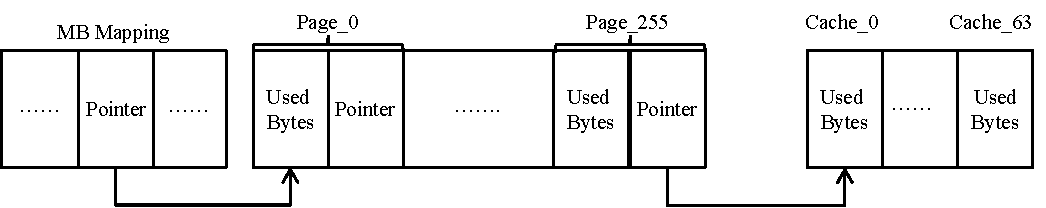
\includegraphics[width=6.3in]{figures/lookup}
\caption{Fast Lookup Mechanism within Shadow Memory.\label{fig:lookup}}
\end{figure*}

\MP{} updates the corresponding metadata upon each allocation and deallocation, and performs the lookup for each sampled event, where both operations could be performed in constant time. For any given address, \MP{} first computes its MB-based index by dividing the address with 1 MB. Every entry of this MB-based mapping will store a pointer pointing to its page-based entries. 
Note that    

\MP{} is designed to adapt to different allocators, which may have different mechanisms to obtain the memory from the OS, such as via \texttt{brk} or \texttt{mmap} system calls separately. Therefore, memory address spaces are scattered along the whole address space of a process, which makes difficult to utilize virtual memory to provide a fast lookup. Based on our observation, \texttt{mmap} system calls always allocate the space starting from 130 TB space (even with ASLR mechanism enabled). Therefore, \MP{} reserved the last 1TB space for the shadow memory of this.   

First, different allocators may require different ranges of virtual memory from the underlying OS. For instance, the Linux allocator's main arena (expanding with \texttt{sbrk} system call) is far from other arenas obtained with \texttt{mmap} system calls. Second, the number of regions ranges from few to successive   
There are multiple factors may affect the design: the default Linux allocator extends its heap differently with the \texttt{sbrk} system call, making one of its heap arena far from other arenas (making it difficult to design the virtual memory)? Secure allocators, such as OpenBSD and DieHarder, may invoke one \texttt{mmap} to obtain one page from the OS. That is, there are a large number of mappings inside the OS. This fact makes some general data structures not suitable to support the fast lookup, such as a hash map or the range tree.
